\documentclass[11pt,a4paper]{article}

\usepackage[utf8]{inputenc}
\usepackage[T1]{fontenc}
\usepackage{mathptmx}
\usepackage[scaled=.9]{helvet}
\usepackage{courier}
\usepackage[margin=2.4cm]{geometry}
\usepackage{amsmath,amssymb,amsthm}
\usepackage{booktabs,longtable,enumitem,verbatim}
\usepackage{xcolor}
\usepackage{microtype}
\usepackage{algorithm}
\usepackage[noend]{algpseudocode}
\usepackage{listings}
\usepackage{tikz}
\usepackage[hidelinks]{hyperref}

% ------------------------------------------------------------------
% Fill in your details here (one place only).
% ------------------------------------------------------------------
\newcommand{\studentname}{[Your name]}
\newcommand{\rollno}{[Roll number]}
\newcommand{\coursename}{Design and Analysis of Algorithms -- Course Project}

% ------------------------------------------------------------------
% The tables and outputs below are produced by running the program while
% this file compiles (pdflatex -shell-escape report.tex).  If shell escape
% is not available (e.g. on Overleaf) the last generated files, which are
% committed to the repository, are used instead.
% ------------------------------------------------------------------
\immediate\write18{python3 lecture_solver.py --latex-report > generated_tests.tex}
\immediate\write18{python3 lecture_solver.py --latex-bench > generated_bench.tex}
\immediate\write18{python3 lecture_solver.py --demo > demo_output.txt}
\immediate\write18{python3 lecture_solver.py sample.txt > sample_output.txt}

\newtheorem{lemma}{Lemma}
\newtheorem{theorem}{Theorem}
\newtheorem{corollary}{Corollary}
\theoremstyle{definition}
\newtheorem{definition}{Definition}
\theoremstyle{remark}
\newtheorem{remark}{Remark}

\newcommand{\Z}{\mathbb{Z}}
\newcommand{\hit}{\mathrm{hit}}
\newcommand{\Qf}{Q}
\newcommand{\Tf}{T}

\lstset{basicstyle=\ttfamily\scriptsize, numbers=left, numberstyle=\tiny\color{gray},
  breaklines=true, columns=fullflexible, keepspaces=true, frame=single,
  commentstyle=\color{gray}, language=Python, showstringspaces=false}

\title{Lecture Supervision on a Circular Timetable:\\
       Efficient Open Domination of a Circular-Arc Graph}
\author{\studentname\ (\rollno)\\[2pt] \coursename}
\date{\today}

\begin{document}
\maketitle

\begin{abstract}
\noindent $n$ lectures repeat every day on a circular timetable of $L=1440$ minutes.
We must choose a set $S$ of lectures such that every lecture overlaps exactly one
lecture of $S$.  This is an \emph{efficient open dominating set} (a total perfect
code) of the circular-arc overlap graph.  We prove that every solution is a union of
disjoint \emph{blocks}, show that there are at most $2n$ candidate blocks, and give
an $O(n^3)$ algorithm that anchors one block, unrolls the circle and runs a dynamic
programme over the remaining blocks.  The algorithm is implemented in Python,
verified by an independent checker, and cross-checked against exhaustive search on
more than a thousand random, planted and mutated instances.  All code is available at
\url{https://github.com/Revanth422/DAA}.
\end{abstract}

\tableofcontents

% ======================================================================
\section{Problem statement and classification}
% ======================================================================
Time is divided into $L=1440$ unit \emph{cells} (minutes) arranged on a circle, so
cell $L-1$ is followed by cell $0$.  Lecture $i$ ($1\le i\le n$) is given by a start
$s_i$ and an end $e_i$ (both in $\{0,\dots,L-1\}$) and occupies the arc
\[
  A_i=\{s_i,\,s_i+1,\,\dots,\,s_i+d_i-1\}\pmod L,\qquad
  d_i=\begin{cases}(e_i-s_i)\bmod L & e_i\ne s_i,\\ L & e_i=s_i,\end{cases}
\]
so a lecture may wrap past midnight, and $s_i=e_i$ denotes a full-day lecture.
Two distinct lectures \emph{overlap} if $A_i\cap A_j\neq\emptyset$, i.e.\ if they share
positive length; lectures that only touch at an endpoint do \emph{not} overlap.
Let $G$ be the overlap graph and $N(v)$ the \emph{open} neighbourhood of $v$ (a lecture
is never its own neighbour).

\paragraph{Task.} Find $S\subseteq\{1,\dots,n\}$ such that $|N(v)\cap S|=1$ for every
lecture $v$, or report that none exists.  Equivalently, the open neighbourhoods
$N(s)$, $s\in S$, partition the vertex set.  Such an $S$ is called an
\emph{efficient open dominating set} or \emph{total perfect code} \cite{cdh,gs}.

\paragraph{Classification.} $G$ is a circular-arc graph \cite{golumbic}.  The problem is
an exact-cover problem, and a brute-force search over all subsets needs $\Theta(2^n)$
candidates.  We exploit the circular structure: a structural characterisation
(Section~\ref{sec:structure}) reduces the search to chains of ``blocks'' around the
circle, which a dynamic programme over a linearised (``anchored'') circle decides in
polynomial time, using bit-set graph operations (technique: structural decomposition
+ dynamic programming \cite{clrs}).

\paragraph{Conventions.} Lectures are numbered $1,\dots,n$ in this report and in the
program output (the source code uses $0,\dots,n-1$ internally).  The complete input
format is described in Section~\ref{sec:impl}.

% ======================================================================
\section{Structure of every solution}\label{sec:structure}
% ======================================================================
\begin{definition}[Block, region, hit]
A \emph{block} is a pair $\{a,b\}$ of overlapping lectures with
$N(a)\cap N(b)=\emptyset$.  Its \emph{region} is $R=A_a\cup A_b$.  A lecture $w$
\emph{hits} a region $R$ if $A_w\cap R\ne\emptyset$ (a lecture of the block hits its
own region).
\end{definition}
Because $a\in N(b)$ and $b\in N(a)$ but $a\notin N(a)$, the condition
$N(a)\cap N(b)=\emptyset$ says exactly that \emph{no third lecture overlaps both $a$
and $b$}.  Consequently, if $w\notin\{a,b\}$ hits the region of a block $\{a,b\}$, then $w$
overlaps \emph{exactly one} of $a,b$.  $(\ast)$

\begin{lemma}[Decomposition]\label{lem:decomp}
A nonempty set $S$ is valid (every lecture overlaps exactly one lecture of $S$) if and
only if $S=B_1\cup\dots\cup B_k$ ($k\ge1$) for pairwise disjoint blocks $B_j$ with
regions $R_j$ such that
\begin{equation}\tag{$\star$}
\text{every lecture hits exactly one of the regions } R_1,\dots,R_k .
\end{equation}
In that case the regions $R_1,\dots,R_k$ are pairwise disjoint.
\end{lemma}
\begin{proof}
($\Rightarrow$) Every $v\in S$ has exactly one neighbour $p(v)\in S$, and
$p(p(v))=v$ because $v$ is a neighbour of $p(v)$ in $S$.  Hence $S$ splits into the pairs
$\{v,p(v)\}$; call them $B_1,\dots,B_k$.  If some $w$ were in $N(a)\cap N(b)$ for
$B_j=\{a,b\}$, then $w$ would have two neighbours in $S$; so each $B_j$ is a block.
Now let $w$ be any lecture.  If $w\notin S$, then $w$ hits $R_j$ iff $w$ overlaps a
lecture of $B_j$; since $w$ has exactly one neighbour in $S$, it hits exactly one
region.  If $w\in B_i$, it hits $R_i$; if it also hit $R_j$, $j\ne i$, it would overlap
some $x\in B_j$ in addition to $p(w)$, a contradiction.  This proves $(\star)$.
Finally, a cell lying in $R_i\cap R_j$ ($i\ne j$) would belong to some $x\in B_i$ and
some $y\in B_j$, so $x$ would hit $R_j$ and $R_i$, contradicting $(\star)$.

($\Leftarrow$) Let $w$ be a lecture and $R_j$ the unique region it hits.  Every
neighbour $x\in S$ of $w$ lies in some $B_i$, and then $w$ hits $R_i$, so $i=j$:
all neighbours of $w$ in $S$ lie in $B_j=\{a,b\}$.  If $w\notin B_j$, then $w$ hits
$R_j$, so it overlaps at least one of $a,b$, and by $(\ast)$ exactly one.  If $w=a$, its
only possible neighbour in $S$ is $b$, and $a$ overlaps $b$.  In all cases $w$ has
exactly one neighbour in $S$.
\end{proof}

\begin{corollary}[Whole-circle block]\label{cor:whole}
If $\{a,b\}$ is a block with $A_a\cup A_b=\Z_L$, then $S=\{a,b\}$ is valid.
\end{corollary}
\begin{proof}
Every lecture has at least one cell, so it hits the single region $\Z_L$ exactly once;
apply Lemma~\ref{lem:decomp}.
\end{proof}

\begin{lemma}[Few blocks]\label{lem:few}
There are at most $2n$ blocks whose region is not the whole circle.
\end{lemma}
\begin{proof}
Let $\{a,b\}$ be a block with $R\ne\Z_L$.  Cut the circle at a cell outside $R$; then
$A_a$ and $A_b$ become ordinary intervals.  They overlap, so exactly one of two cases
occurs.

\emph{Nested.} One arc contains the other, say $A_b\subseteq A_a$ (if the arcs are equal,
let $b$ be the lecture with the larger index).  Every lecture touching $b$ touches $a$,
so $N(b)\setminus\{a\}\subseteq N(a)\cap N(b)=\emptyset$, i.e.\ $N(b)=\{a\}$.  Thus
$b$ determines $a$, and there are at most $n$ nested blocks.

\emph{Crossing.} Neither arc contains the other, so in the cut picture
$s_a<s_b<e_a<e_b$ (after naming).  Exactly one of the two lectures, here $a$, has its
\emph{last cell} inside the other arc; call it the \emph{left} member (this notion does
not depend on where the circle was cut).  Suppose $a$ is the left member of two
different blocks $\{a,b\}$ and $\{a,b'\}$.  The last cell $c$ of $a$ lies in $A_b$ and
in $A_{b'}$.  Then $b'$ overlaps $a$ and overlaps $b$ (both contain $c$), so
$b'\in N(a)\cap N(b)$, contradicting that $\{a,b\}$ is a block.  Hence every lecture is
the left member of at most one crossing block, giving at most $n$ crossing blocks.
\end{proof}

% ======================================================================
\section{The algorithm}\label{sec:algo}
% ======================================================================
\paragraph{Idea.} By Lemma~\ref{lem:decomp}, lecture~1 hits exactly one region in any
solution, i.e.\ it belongs to or touches exactly one block.  We try every candidate
block that hits lecture~1 as an \emph{anchor}, rotate the circle so that the anchor's
region starts at coordinate $0$, unroll the circle to the line $[0,L]$, and decide with a
left-to-right dynamic programme whether the remaining blocks can be chained so that
$(\star)$ holds.

\paragraph{Coordinates.} For an anchor region $R_0=[0,\ell_0)$, lecture $j$ is placed at
start $\sigma_j\in[0,L)$ (relative to the anchor) with end $\varepsilon_j=\sigma_j+d_j$.
Besides $[\sigma_j,\varepsilon_j)$ we also use the copy $[\sigma_j-L,\varepsilon_j-L)$ that
accounts for lectures crossing the anchor's start.  For a position $p$ define
\begin{align*}
 \Qf(p)&=\max\bigl(\{\varepsilon_j:\sigma_j<p\}\cup\{\varepsilon_j-L:\text{all }j\}\bigr)
   &&\text{(furthest end of a lecture copy starting before $p$)},\\
 \Tf(p)&=\min\{\varepsilon_j:\sigma_j\ge p\}\quad(\min\emptyset=\infty)
   &&\text{(earliest end of a lecture starting at or after $p$)}.
\end{align*}
Both are computed for all $p$ in $O(n\log n)$ by sorting once and using a prefix
maximum and a suffix minimum.

\paragraph{Chains.} A \emph{chain} is a sequence of blocks $X_0,\dots,X_{k-1}$
($X_0$ the anchor) whose regions are arcs $[\alpha_i,\beta_i)$ with
\[
 0=\alpha_0<\beta_0\le\alpha_1<\beta_1\le\dots\le\alpha_{k-1}<\beta_{k-1}\le L=:\alpha_k .
\]
The \emph{gap} $G_i=[\beta_i,\alpha_{i+1})$ (possibly empty) lies between $X_i$ and the
next region; $G_{k-1}$ leads back to the anchor.  A chain satisfies the \emph{gap tests}
if
\begin{align}
 &\Tf(\beta_i)>\alpha_{i+1} &&\text{for all } i\in\{0,\dots,k-1\}
   &&\text{(no lecture lies strictly inside a gap)},\tag{G1}\\
 &\Qf(\beta_i)\le\alpha_{i+1} &&\text{for all } i\text{, if }k\ge2
   &&\text{(no lecture meets two consecutive regions)}.\tag{G2}
\end{align}
For $k=1$ only (G1) is needed.

\begin{lemma}[Chain lemma]\label{lem:chain}
For a chain as above, every lecture hits exactly one of the regions
$R_i=[\alpha_i,\beta_i)$ if and only if (G1) and (G2) hold.
\end{lemma}
\begin{proof}
The cells $[0,L)$ are the disjoint union $R_0\cup G_0\cup R_1\cup\dots\cup R_{k-1}\cup G_{k-1}$.

\emph{No lecture hits no region $\iff$ (G1).}  A lecture hits no region iff its arc is
contained in the union of the gaps.  An arc is contiguous and the gaps are separated by
regions, so it lies inside a single gap $G_i$ (the last gap is followed, cyclically, by
cell $0\in R_0$).  Then it does not wrap, so it has $\sigma_j\ge\beta_i$ and
$\varepsilon_j\le\alpha_{i+1}$, whence $\Tf(\beta_i)\le\alpha_{i+1}$.  Conversely, if
$\Tf(\beta_i)\le\alpha_{i+1}$ then the lecture attaining the minimum satisfies
$\sigma_j\ge\beta_i$ and $\varepsilon_j\le\alpha_{i+1}$, i.e.\ lies inside $G_i$.

\emph{No lecture hits two regions $\iff$ (G2) (for $k\ge2$).}  If a copy of a lecture
satisfies $\sigma<\beta_i$ and $\varepsilon>\alpha_{i+1}$, it contains the cells
$\beta_i-1\in R_i$ and $\alpha_{i+1}$, which lies in $R_{i+1}$ (or equals $L\equiv0\in R_0$
when $i=k-1$); for $k\ge2$ these are different regions.  Such a copy exists iff
$\Qf(\beta_i)>\alpha_{i+1}$.  Conversely, suppose a lecture contains a cell $x\in R_u$
and a cell $y\in R_v$ with $u\ne v$.  Its arc contains one of the two cyclic paths from
$x$ to $y$; say (after exchanging the names of $x,y$) the path that moves forward from
$x$.  Leaving $R_u$ the path passes through $\beta_u-1$ and reaches the first cell
$\alpha_{u+1}$ of the next region before reaching $y$.  So the arc contains all cells from
$\beta_u-1$ to $\alpha_{u+1}$, and the copy of the lecture that does so has
$\sigma<\beta_u$ and $\varepsilon>\alpha_{u+1}$: (G2) fails for $i=u$.

Hitting exactly one region means hitting neither none nor two or more; this is
(G1)$\wedge$(G2).
\end{proof}

\paragraph{Dynamic programme.} Let $C$ be the list of candidate blocks whose region lies
in $[\ell_0,L]$ (these are exactly the blocks whose region is disjoint from $R_0$),
sorted by start $\alpha$.  Write $\mathrm{reach}[Y]$ for ``there is a chain $X_0,\dots,Y$
satisfying (G1), (G2) between all consecutive blocks''.  Then
\[
 \mathrm{reach}[X_0]=\text{true},\qquad
 \mathrm{reach}[Y]=\exists X\text{ before }Y:\ \mathrm{reach}[X]\wedge\beta_X\le\alpha_Y\wedge
 \Qf(\beta_X)\le\alpha_Y<\Tf(\beta_X),
\]
and the chain closes at $Y$ if $\Qf(\beta_Y)\le L<\Tf(\beta_Y)$.  The case $k=1$ is
the test $L<\Tf(\ell_0)$.

\begin{algorithm}[t]
\caption{\textsf{SelectLectures}(lectures, $L$)}\label{alg:main}
\begin{algorithmic}[1]
\State build bit-masks of covered minutes and adjacency bit-sets $N(\cdot)$
\State $\mathcal B\gets\{\{a,b\}: a\cap b\ne\emptyset,\ N(a)\cap N(b)=\emptyset\}$
\If{some block of $\mathcal B$ covers the whole circle} \State \Return it
  \Comment{Corollary~\ref{cor:whole}}
\EndIf
\ForAll{$X_0\in\mathcal B$ whose region hits lecture 1}\Comment{anchors}
  \State rotate so that $X_0=[0,\ell_0)$; compute $\Qf,\Tf$ by prefix max / suffix min
  \State $C\gets$ blocks lying in $[\ell_0,L]$, sorted by start
  \If{$L<\Tf(\ell_0)$} \State \Return $X_0$ \Comment{$k=1$}
  \EndIf
  \ForAll{$Y\in C$ in order of start}
    \State $\mathrm{reach}[Y]\gets\exists X\in\{X_0\}\cup C$ before $Y$ with $\mathrm{reach}[X]$,
      $\beta_X\le\alpha_Y$, $\Qf(\beta_X)\le\alpha_Y<\Tf(\beta_X)$
    \If{$\mathrm{reach}[Y]$ \textbf{and} $\Qf(\beta_Y)\le L<\Tf(\beta_Y)$}
      \State \Return the chain ending in $Y$
    \EndIf
  \EndFor
\EndFor
\State \Return \textsf{None}
\end{algorithmic}
\end{algorithm}

\paragraph{Worked example (test T4).} Lectures (times in hours):
L1 0--2, L2 1--3, L3 0:30--1, L4 8--10, L5 9--11, L6 8:30--9, L7 16--18, L8 17--19.
The first anchor meeting lecture~1 is $X_0=\{L1,L2\}$ with region $[0,180)$ minutes
(00:00--03:00).  The other blocks inside $[180,1440]$ include $Y_1=\{L4,L6\}$ with
region $[480,600)$ and $Y_2=\{L7,L8\}$ with region $[960,1140)$.  The tests are:
\begin{center}
\begin{tabular}{llccc}
\toprule
Transition & values & $\Qf(\beta)\le\alpha$ & $\alpha<\Tf(\beta)$ & result\\
\midrule
$X_0\to Y_1$ & $\Qf(180)=180,\ \alpha=480,\ \Tf(180)=540$ & \checkmark & \checkmark & ok\\
$Y_1\to Y_2$ & $\Qf(600)=660,\ \alpha=960,\ \Tf(600)=1080$ & \checkmark & \checkmark & ok\\
$Y_2\to X_0{+}L$ & $\Qf(1140)=1140,\ \alpha=1440,\ \Tf(1140)=\infty$ & \checkmark & \checkmark & closes\\
\bottomrule
\end{tabular}
\end{center}
Hence the chain $X_0,Y_1,Y_2$ is accepted and $S=\{1,2,4,6,7,8\}$ is returned, exactly the
output of the program (Appendix~\ref{app:out}).  Figure~\ref{fig:t4} shows the instance:
the selected lectures are dark, the shaded bands are the three regions.

\begin{figure}[t]
\centering
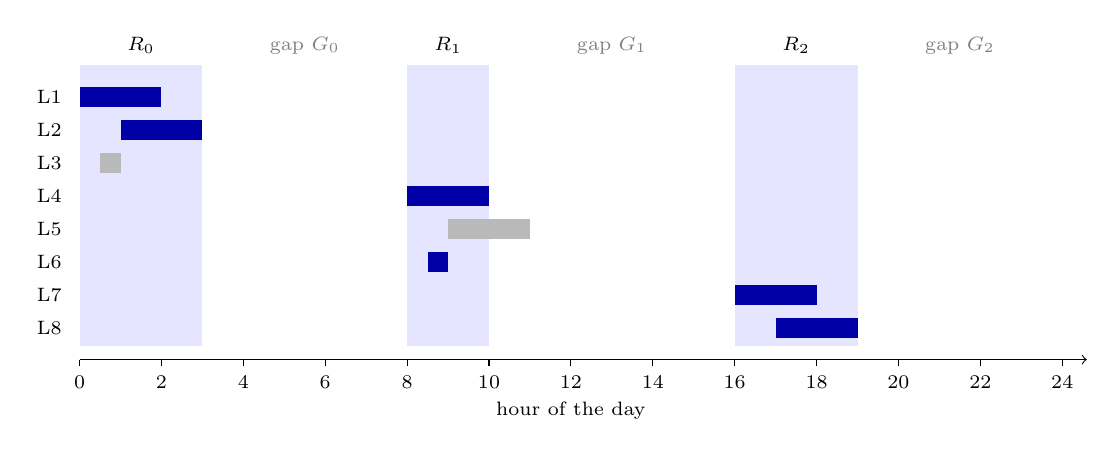
\begin{tikzpicture}[x=0.52cm,y=0.42cm,font=\scriptsize]
  \fill[blue!10] (0,0.3) rectangle (3,-8.2);
  \fill[blue!10] (8,0.3) rectangle (10,-8.2);
  \fill[blue!10] (16,0.3) rectangle (19,-8.2);
  \node at (1.5,0.9) {$R_0$};  \node at (9,0.9) {$R_1$};  \node at (17.5,0.9) {$R_2$};
  \node[gray] at (5.5,0.9) {gap $G_0$};
  \node[gray] at (13,0.9) {gap $G_1$};
  \node[gray] at (21.5,0.9) {gap $G_2$};
  \foreach \i/\s/\e/\sel in {1/0/2/1, 2/1/3/1, 3/0.5/1/0, 4/8/10/1,
                             5/9/11/0, 6/8.5/9/1, 7/16/18/1, 8/17/19/1} {
    \pgfmathsetmacro{\yt}{-\i+0.65}
    \pgfmathsetmacro{\yb}{-\i+0.05}
    \ifnum\sel=1
      \fill[blue!65!black] (\s,\yt) rectangle (\e,\yb);
    \else
      \fill[gray!55] (\s,\yt) rectangle (\e,\yb);
    \fi
    \node[left] at (-0.2,{-\i+0.35}) {L\i};
  }
  \draw[->] (0,-8.6) -- (24.6,-8.6);
  \foreach \h in {0,2,...,24} {\draw (\h,-8.6) -- (\h,-8.8) node[below] {\h};}
  \node[below] at (12,-9.6) {hour of the day};
\end{tikzpicture}
\caption{Test T4. Dark bars: selected lectures $\{1,2,4,6,7,8\}$; grey bars: lectures that
are not selected (L3, L5).  Shaded bands: regions of the chain $X_0,Y_1,Y_2$.}
\label{fig:t4}
\end{figure}

% ======================================================================
\section{Correctness}\label{sec:correct}
% ======================================================================
\begin{theorem}\label{thm:main}
\textsf{SelectLectures} returns a valid subset if one exists and \textsf{None} otherwise.
\end{theorem}
\begin{proof}
\emph{Soundness.} Suppose a set is returned.  If it comes from the whole-circle case it
is valid by Corollary~\ref{cor:whole}.  Otherwise it is the union of the blocks of a
chain.  The filter ``region inside $[\ell_0,L]$'' together with the condition
$\beta_X\le\alpha_Y$ makes the regions pairwise disjoint and ordered, so the chain is as
in Section~\ref{sec:algo}; the accepted transitions and the closing test are exactly
(G1) and (G2) for all gaps (for $k=1$: (G1) only).  By Lemma~\ref{lem:chain} every
lecture hits exactly one region, and by Lemma~\ref{lem:decomp} ($\Leftarrow$) the union of
the blocks is valid.

\emph{Completeness.} Let $S$ be valid.  If $S$ contains a block whose region is the
whole circle, then $k=1$ (any other region would be hit twice) and the special case
returns a valid block.  Otherwise let $B_1,\dots,B_k$ be the blocks of $S$ from
Lemma~\ref{lem:decomp}; their regions are pairwise disjoint arcs, and lecture~1 hits
exactly one of them, say $R_1$.  Block $B_1$ is therefore among the anchors tried.  With
$B_1$ rotated to coordinate $0$, every other region is an arc disjoint from
$R_1=[0,\ell_0)$, hence lies in $[\ell_0,L]$ and is in the list $C$; ordering them by
start gives the cyclic order, i.e.\ a chain $X_0=B_1,X_1,\dots,X_{k-1}$.  By $(\star)$
and Lemma~\ref{lem:chain}, (G1) and (G2) hold along it.  If $k=1$ the test
$L<\Tf(\ell_0)$ succeeds.  If $k\ge2$, induction along the chain shows
$\mathrm{reach}[X_i]$ becomes true (the true predecessor $X_{i-1}$ passes the
transition test, although the DP may record a different valid predecessor), and the
closing test succeeds at $X_{k-1}$ (or at an earlier block, which is again valid by
soundness).  So some anchor returns a chain, and the algorithm does not output
\textsf{None}.
\end{proof}

% ======================================================================
\section{Complexity}\label{sec:complexity}
% ======================================================================
Let $w$ be the machine word size (the program uses Python integers as bit-sets).
\begin{itemize}[nosep]
 \item \emph{Masks and adjacency.} $n$ masks of $L$ bits and $\binom n2$ intersections
   cost $O(n^2L/w)$.  For the fixed $L=1440$ this is a constant factor of about
   $1440/64\approx23$ word operations per pair.
 \item \emph{Blocks.} Each of the $O(n^2)$ pairs needs one $n$-bit intersection
   $N(a)\cap N(b)$, i.e.\ $O(n^3/w)$ in total.
 \item \emph{Number of blocks.} If a block covers the whole circle we stop.  Otherwise there
   are $m\le2n$ blocks by Lemma~\ref{lem:few}, hence at most $2n$ anchors.
 \item \emph{One anchor.} Sorting and computing $\Qf,\Tf$ costs $O(n\log n)$; the DP
   examines all pairs of blocks, $O(m^2)=O(n^2)$.
\end{itemize}
Altogether
\[
 T(n)=O\!\left(n^2L/w+n^3\right)=O(n^3)\ \text{for fixed }L,\qquad
 S(n)=O(n^2+nL)\ \text{bits}=O(n^2)\text{ bits for fixed }L.
\]
(The $nL$ term is linear in $n$, not constant; for $L=1440$ it is dominated by $n^2$ as soon
as $n>1440$.)  This is polynomial, compared with $\Theta(2^n)$ subsets for exhaustive
search.  The cubic bound is an upper bound; Section~\ref{sec:exp} measures the actual
growth.

% ======================================================================
\section{Implementation and reproducibility}\label{sec:impl}
% ======================================================================
\paragraph{Source code.} The complete Python implementation, the sample input and a
README are in the public repository

\begin{center}\url{https://github.com/Revanth422/DAA}\end{center}

\noindent (the solver itself: \url{https://github.com/Revanth422/DAA/blob/main/lecture_solver.py}).
The repository contains \texttt{lecture\_solver.py} (algorithm, independent verifier,
brute-force checker, test generators, benchmark), \texttt{sample.txt} and
\texttt{mydata.txt} (example inputs), \texttt{README.md}, this report's LaTeX source
\texttt{report.tex} with its generated files, and a GitHub Actions workflow that runs the
tests on every push.  The listing in Appendix~\ref{app:src} is read directly from
\texttt{lecture\_solver.py} when this document is built, so it is always the file that
produced the results.

\paragraph{Input format.} The first line contains $n$; then $n$ lines
\texttt{HH:MM HH:MM} (start, end; 24-hour clock, \texttt{24:00} means midnight).  Text after
\texttt{\#} is a comment.  Plain integers are read as minutes after midnight.
\texttt{mydata.txt} is simply an example of such a file for the reader's own data:
\begin{center}\ttfamily\small
\begin{tabular}{l}
4\\ 23:00 01:00\\ 00:30 02:00\\ 13:00 15:00\\ 14:00 16:00
\end{tabular}
\end{center}

\paragraph{Running.}
\begin{center}\ttfamily\small
\begin{tabular}{ll}
python3 lecture\_solver.py sample.txt & solve an input file\\
python3 lecture\_solver.py --demo & the 8 built-in tests\\
python3 lecture\_solver.py --stress 1000 & compare with brute force\\
python3 lecture\_solver.py --bench & running times\\
pdflatex -shell-escape report.tex & rebuild this PDF (runs the code)
\end{tabular}
\end{center}

\paragraph{Independent verification.} The solver works on a bit-mask graph.  The checker
\texttt{verify} and the exhaustive search \texttt{brute\_force} do \emph{not} reuse it:
they decide overlap with the arithmetic test ``arc $A$ contains the start cell of arc $B$,
or vice versa'' (two cyclic arcs intersect iff one contains the other's first cell).  A
wrong overlap model in the solver would therefore be detected.  The stress tests also check that the
bit-mask graph and the arithmetic graph are identical.

% ======================================================================
\section{Experiments}\label{sec:exp}
% ======================================================================
\subsection{Built-in tests and cross-checks}
The following table is produced by the program while this document compiles.  Each row
runs the solver, the exhaustive search and the independent verifier.

\IfFileExists{generated_tests.tex}{\begin{longtable}{p{4.6cm}p{5.6cm}p{2.6cm}c}
\toprule Test & Lectures (start--end) & Algorithm output & OK \\ \midrule \endhead
T1 two overlapping lectures & {\footnotesize L1\,09:00--10:00, L2\,09:30--10:30} & $S=\{1,2\}$ & \checkmark \\
T2 night lecture wraps midnight & {\footnotesize L1\,23:00--01:00, L2\,00:30--02:00} & $S=\{1,2\}$ & \checkmark \\
T3 two chains around the day & {\footnotesize L1\,01:00--03:00, L2\,02:00--04:00, L3\,13:00--15:00, L4\,14:00--16:00} & $S=\{1,2,3,4\}$ & \checkmark \\
T4 four blocks, private lectures & {\footnotesize L1\,00:00--02:00, L2\,01:00--03:00, L3\,00:30--01:00, L4\,08:00--10:00, L5\,09:00--11:00, L6\,08:30--09:00, L7\,16:00--18:00, L8\,17:00--19:00} & $S=\{1,2,4,6,7,8\}$ & \checkmark \\
T5 lecture touched by two blocks & {\footnotesize L1\,01:00--03:00, L2\,02:00--04:00, L3\,05:00--07:00, L4\,06:00--08:00, L5\,03:30--05:30} & none & \checkmark \\
T6 full-day lecture + private partner & {\footnotesize L1\,00:00--00:00, L2\,10:00--11:00} & $S=\{1,2\}$ & \checkmark \\
T7 isolated lecture & {\footnotesize L1\,09:00--10:00, L2\,09:30--10:30, L3\,15:00--16:00} & none & \checkmark \\
T8 touching endpoints do not overlap & {\footnotesize L1\,09:00--10:00, L2\,10:00--11:00} & none & \checkmark \\
\bottomrule \end{longtable}
\begin{center}\begin{tabular}{lrrr}
\toprule Instance family & Instances & Solvable & Disagreements \\ \midrule
random, period 24 & 200 & 35 & 0 \\
planted, period 24 & 200 & 200 & 0 \\
mutated, period 24 & 200 & 92 & 0 \\
planted, period 1440 & 200 & 200 & 0 \\
mutated, period 1440 & 200 & 88 & 0 \\
\bottomrule \end{tabular}\end{center}
\par\noindent\textbf{All built-in tests and all cross-checks passed.}
}{\textbf{(generated\_tests.tex missing: run \texttt{python3 lecture\_solver.py --latex-report > generated\_tests.tex})}}

The tests cover wrap-around at midnight (T2), several blocks with private lectures (T4),
a lecture touched by two blocks (T5), a full-day lecture (T6), an isolated lecture (T7)
and lectures that merely touch at an endpoint (T8).  The random families compare the
polynomial algorithm with exhaustive search (up to 10 lectures).  \emph{Planted}
instances are solvable by construction (random blocks, crossing or nested, with
private lectures, randomly rotated and shuffled), so they test the ``yes'' answers;
\emph{mutated} instances change one endpoint, add or delete a lecture of a planted
instance, and are close to the boundary between ``yes'' and ``no''.  All random
instances use fixed seeds and are therefore reproducible.

\subsection{Running time}
We measure \texttt{solve} for $L=1440$ on two families.  \emph{Solvable}: planted
instances.  \emph{Worst case}: lecture~1 is a half-day arc containing $n/2$ tiny private
lectures, so about $n/2$ blocks meet lecture~1 (many anchors); the other half-day holds
about $n/4$ blocks and one isolated lecture makes the instance unsolvable, so the DP
runs for every anchor.
\begin{center}
\IfFileExists{generated_bench.tex}{\begin{center}\begin{tabular}{rrrrr}
\toprule $n$ & solvable: time (s) & $n$ & worst case: time (s) & growth \\ \midrule
100 & 0.001 & 100 & 0.005 & -- \\
200 & 0.003 & 200 & 0.025 & $\times4.7$ \\
400 & 0.013 & 400 & 0.129 & $\times5.2$ \\
800 & 0.047 & 800 & 0.716 & $\times5.5$ \\
\bottomrule \end{tabular}\end{center}
}{\textbf{(generated\_bench.tex missing)}}
\end{center}
Doubling $n$ multiplies the time by a factor of roughly $4$ to $7$ on the adversarial family,
between the factors $4$ (quadratic) and $8$ (cubic).  The $O(n^3)$ bound is thus an upper bound
which the experiment does not contradict; whether it is tight is left open.  Times are
machine dependent and were measured on the machine that built this PDF.

% ======================================================================
\section{Conclusion and limitations}
% ======================================================================
Every solution is a disjoint union of blocks, only $O(n)$ blocks can be candidates, and
anchoring one block turns the circular problem into a linear dynamic programme.  The algorithm runs in $O(n^3)$
time, is proved correct and agrees with exhaustive search on all tested instances.
Limitations: time is discretised to whole minutes (the model with real-valued endpoints is
analogous but would need coordinate compression); the cubic bound may not be tight; and the
random cross-checks are limited by the exponential cost of the reference solver to small $n$.
A natural improvement is to replace the $L$-bit masks by $O(1)$ arithmetic overlap tests.

\begin{thebibliography}{9}
\bibitem{clrs} T.~H.~Cormen, C.~E.~Leiserson, R.~L.~Rivest, C.~Stein,
\emph{Introduction to Algorithms}, 4th ed., MIT Press, 2022.
\bibitem{cdh} E.~J.~Cockayne, R.~M.~Dawes, S.~T.~Hedetniemi,
Total domination in graphs, \emph{Networks} 10 (1980), 211--219.
\bibitem{gs} H.~Gavlas, K.~Schultz, Efficient open domination,
\emph{Electronic Notes in Discrete Mathematics} 11 (2002).
\bibitem{golumbic} M.~C.~Golumbic, \emph{Algorithmic Graph Theory and Perfect Graphs},
2nd ed., Elsevier, 2004.
\end{thebibliography}

\appendix
\section{Raw program output}\label{app:out}
Output of \texttt{python3 lecture\_solver.py --demo} (the eight built-in tests):
{\footnotesize
\IfFileExists{demo_output.txt}{\verbatiminput{demo_output.txt}}{(demo\_output.txt missing)}}

\noindent Output of \texttt{python3 lecture\_solver.py sample.txt}:
{\footnotesize
\IfFileExists{sample_output.txt}{\verbatiminput{sample_output.txt}}{(sample\_output.txt missing)}}

\section{Source code}\label{app:src}
The complete file \texttt{lecture\_solver.py}:
\lstinputlisting{lecture_solver.py}

\end{document}
